%%
%% This is file `main.tex' based on `sample-sigconf.tex' (q.v. for spurce of that,
%%
%% IMPORTANT NOTICE:
%% 
%% For the copyright see the original source file `sample-sigconf.tex'
%% in the `Sample' folder.
%%
%% For distribution of the original source see the terms
%% for copying and modification in the file samples.dtx.
%% 
%% This generated file may be distributed as long as the
%% original source files, as listed above, are part of the
%% same distribution. (The sources need not necessarily be
%% in the same archive or directory.)
%%
%% Commands for TeXCount
%TC:macro \cite [option:text,text]
%TC:macro \citep [option:text,text]
%TC:macro \citet [option:text,text]
%TC:envir table 0 1
%TC:envir table* 0 1
%TC:envir tabular [ignore] word
%TC:envir displaymath 0 word
%TC:envir math 0 word
%TC:envir comment 0 0
%%
%%
%% The first command in your LaTeX source must be the \documentclass command.

%% NOTE that a single column version is required for 
%% submission and peer review. This can be done by changing
%% the \doucmentclass[...]{acmart} in this template to 
%%\documentclass[manuscript,review,anonymous]{acmart}
%% This version is used for drafting and final submission
\documentclass[sigconf]{acmart}


%% 
%% To ensure 100% compatibility, please check the white list of
%% approved LaTeX packages to be used with the Master Article Template at
%% https://www.acm.org/publications/taps/whitelist-of-latex-packages 
%% before creating your document. The white list page provides 
%% information on how to submit additional LaTeX packages for 
%% review and adoption.
%% Fonts used in the template cannot be substituted; margin 
%% adjustments are not allowed.

%%
%% Submission ID.
%% Use this when submitting an article to a sponsored event. You'll
%% receive a unique submission ID from the organizers
%% of the event, and this ID should be used as the parameter to this command.
%%\acmSubmissionID{123-A56-BU3}

%%
%% For managing citations, it is recommended to use bibliography
%% files in BibTeX format.
%%
%% You can then either use BibTeX with the ACM-Reference-Format style,
%% or BibLaTeX with the acmnumeric or acmauthoryear sytles, that include
%% support for advanced citation of software artefact from the
%% biblatex-software package, also separately available on CTAN.
%%
%% Look at the sample-*-biblatex.tex files for templates showcasing
%% the biblatex styles.
%%

%%
%% The majority of ACM publications use numbered citations and
%% references.  The command \citestyle{authoryear} switches to the
%% "author year" style.
%%
%% If you are preparing content for an event
%% sponsored by ACM SIGGRAPH, you must use the "author year" style of
%% citations and references.
%% Uncommenting
%% the next command will enable that style.
%%\citestyle{acmauthoryear}

%%
%% end of the preamble, start of the body of the document source.

%% % Location of your graphics files for figures, here a sub-folder to the main project folder
\graphicspath{{./images/}} 

\begin{document}

%%
%% The "title" command has an optional parameter,
%% allowing the author to define a "short title" to be used in page headers.
\title{Ghost in the Shell - Using Runtime Profiling and LLMs for Code Improvement}

%%
%% The "author" command and its associated commands are used to define
%% the authors and their affiliations.
%% Of note is the shared affiliation of the first two authors, and the
%% "authornote" and "authornotemark" commands
%% used to denote shared contribution to the research.
\author{Connor Wilkinson}
\email{wilkincr@umich.edu}

\author{Fardeen Ahmed}
\email{afardeen@umich.edu}

\author{Kazu Sakamoto}
\email{kazus@umich.edu}

\author{Joe Ghezzi}
\email{jghezzi@umich.edu}

%%
%% By default, the full list of authors will be used in the page
%% headers. Often, this list is too long, and will overlap
%% other information printed in the page headers. This command allows
%% the author to define a more concise list
%% of authors' names for this purpose.
\renewcommand{\shortauthors}{Wilkinson, Ahmed, Sakamoto, Ghezzi}

%%
%% The abstract is a short summary of the work to be presented in the
%% article.
\begin{abstract}
  Large language models (LLMs) have become an increasingly popular tool for developers to develop and debug programs. 
  However, for complex programs it is hard for LLMs to identify failures or areas for improvement solely using source code as input.
  Adding runtime information to prompts can improve the quality of LLMs' responses, but this requires significant developer
  time to parse logs. 
  To increase LLM effectiveness and improve ease of use for developers, we present the framework Ghost in the Shell (GinS).
  GinS runs in a thread along an application and collects runtime information, which is then used to automatically 
  construct effective prompts for an LLM.
  LLM analysis can be provided upon program termination, or can be triggered automatically using our novel extension of the existing
  "assert" debugging tool, the smart assert. A developer can insert smart asserts into their code to automatically trigger LLM analysis
  upon assert failure of how the program's runtime behavior caused that assert to fail. [insert more about evaluation]
\end{abstract}

%%
%% This command processes the author and affiliation and title
%% information and builds the first part of the formatted document.
\maketitle

\section{Introduction}
Large Language Models (LLMs) have rapidly become a powerful aid for developers seeking assistance with coding, debugging, and software analysis. 
Recent advancements have shown that LLMs are highly capable of understanding source code and suggesting improvements. 
However, for complex or dynamic software systems, source code alone often lacks sufficient context for effective diagnosis or optimization. 
Developers must typically invest significant time parsing runtime logs and program outputs to supply an LLM with the additional information needed for high-quality feedback.
This reliance on manual log interpretation presents a major bottleneck: while LLMs offer potential to accelerate debugging and program comprehension, the overhead of preparing detailed runtime information can outweigh their benefits. 
Bridging this gap between static code and dynamic behavior remains an open challenge in improving LLM effectiveness for real-world software development tasks.
To address this, we present Ghost in the Shell (GinS), a lightweight framework designed to streamline and automate the integration of runtime data into LLM-assisted workflows. 
GinS operates alongside a target application, continuously collecting relevant runtime information in a non-intrusive thread. 
Upon program termination - or triggered dynamically during execution via our novel smart assert extension - GinS compiles the collected data into rich, targeted prompts for LLMs. 
These prompts enable significantly more accurate and actionable analysis without requiring manual effort from the developer.
Our smart assert mechanism extends traditional assertion tools by not only detecting program failures, but also automatically capturing the runtime state that contributed to the failure. This allows LLMs to provide immediate, context-sensitive feedback on the causes of runtime errors, making debugging faster and more intuitive.
Through evaluation across [insert a short preview of your evaluation here - e.g., benchmarks, case studies, examples], we demonstrate that GinS improves the quality of LLM responses, reduces developer workload, and integrates naturally into existing development practices.

\section{Background}

\begin{figure}
    \centering
    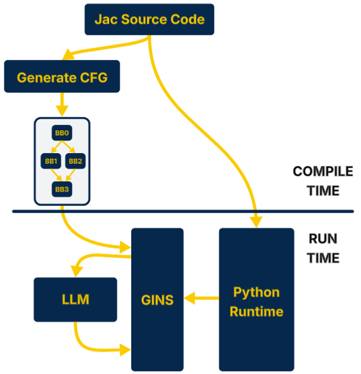
\includegraphics[width=0.5\linewidth]{images/Picture1.png}
    \caption{Design of original implementation of GinS. Note analysis occuring both at compile time and runtime.}
    \label{fig:layout}
\end{figure}

This project is implemented upon a previous CSE 583 semeseter project entitled Ghost in the Shell: A Framework to Prompt LLMs at Runtime with Dynamic Information.
In this project, the group developed a Ghost in the Shell (GinS) thread in the Jac programming language.
The general design of this project can be seen in Figure~\ref{fig:layout}.
Before the target program began (i.e. during compile time), GinS would construct a CFG for the program.
The GinS thread would then run alongside a Python runtime and gather profiling data on it.
This data would then be used to prompt an LLM in real time to request improvement recommendations as well as hot path analysis and error detection.
Our goal in the project discussed in this paper was to provide more detailed analysis of the GinS performance as well as expand its capabilities both in profiling information collected as well as how that information is used.

\section{Expansions on GinS}

\subsection{Additional Runtime Metrics}
The original GinS implementation used its compilation-time CFG to gather basic block execution counts and branch frequencies.
GinS was enabled to collect additional metrics.
One such new metric was time spent in each basic block.
This was to enable bottleneck analysis and other timing analyses.
Another new metric was the most common variable values for a basic block.
The values seen for the variables in that basic block were recorded and this information was used when prompting the LLM.

\subsubsection{Tracing Granularity}
The original GinS implementation only used one type of tracing granularity.
This involved a callback function that was called each time an instruction was executed in the Python runtime.
This enabled very fine granularity, but resulted in significant overhead.
An additional level of tracing granularity was tried in this iteration of the project.
This involved using a timer as a signal to call a profiling function. This lead to lower granularity but also significantly lower overhead.
These tracing granularities were relevant to which profiling metrics were able to be recorded.

\subsection{Updated Prompt Formatting}

\begin{figure}
    \centering
    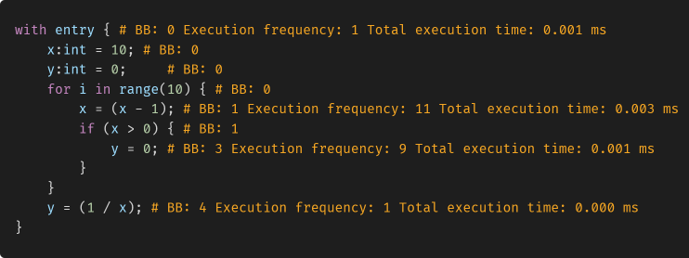
\includegraphics[width=1\linewidth]{images/Picture2.png}
    \caption{Example of source code annotated with basic blocks and execution frequency.}
    \label{fig:annotations}
\end{figure}

A major factor in receiving a quality response from an LLM is prompt design.
It is not just the information that is sent to an LLM that matters; how that information is sent is also highly relevant to response quality.
Because of this, we tested a variety of prompt formats to see which arrangement of information lead to the most useful LLM responses.
There were 5 main prompt types that we used.
For each prompt type, the LLM would be send that type's annotated source code and then an identical prompt.
The first prompt type was plain source code.
The second was the source code annotated with Basic Block values and execution frequencies at each line.
Comments were used to make these annotations (see Figure~\ref{fig:annotations}).
The third prompt type was to annotate the source code with the bytecode instructions that corresponded to each line of python code.
These were annotated in a very similar fashion to the basic block annotations, as were all further discussed annotations.
The fourth prompt type included annotations for the most common seen variable values at each line.
The fifth prompt type included all of the three previously discussed types of annotations, and is referred to as the Combined Complete Information annotation.

\subsection{Smart Assertions}
Smart Assertions, elsewhere referred to as Intelligent Failure Analysis, are an updated form of assert statements.
While a normal assertion statement will print out a previously formed error statement, smart assertions involve taking the runtime state at the time of the assertion failure, submitting it to an LLM, and requesting an analysis for the cause of the failure.
Smart assertions were implemented as function, \texttt{smart\_assert(condition)}, and when imported into a file, could be used as a replacement to standard assertions. When the condition within the smart assert fails, the function interacts with the active GINS instance and calls a final cfg update.
Smart assert then uses the program's source code with its up-to-date runtime annotations to prompt an LLM for analysis on why failure occurred.
The LLMs response is then given to the user through the console before an 'AssertionError' is raised, terminating the program like a standard assert would.

\section{Evaluation}
\subsection{Prompt Formatting Performance}

Seven benchmark programs were used to test the performance of GinS.
These were programs that were solutions to LeetCode problems that contained errors.
Because of this, these programs were not long-running and were not significantly complicated.

For each benchmark, each type of code annotation was created and submitted with a prompt requesting recommendations for code improvement to the Gemini-1.5-pro model.
This model supports structured output.
Thus, a response structure was provided for the model to fill in.
This structure was an array of improvements, where each improvement contained a "start\_line", "end\_line", "type\_of\_improvement", and "improvement\_desc".
start\_line and end\_line corresponded to the start and end of where the code improvement would take place.
type\_of\_improvement was initially an enumerated value with limited types of improvements being able to be suggested by the LLM.
However, this appeared to greatly limit the responses from the LLM.
Thus, this became an open ended value for the LLM to fill in as it saw fit for the given improvement.
improvement\_desc was a field for the LLM to describe the improvement itself.

\begin{figure}
    \centering
    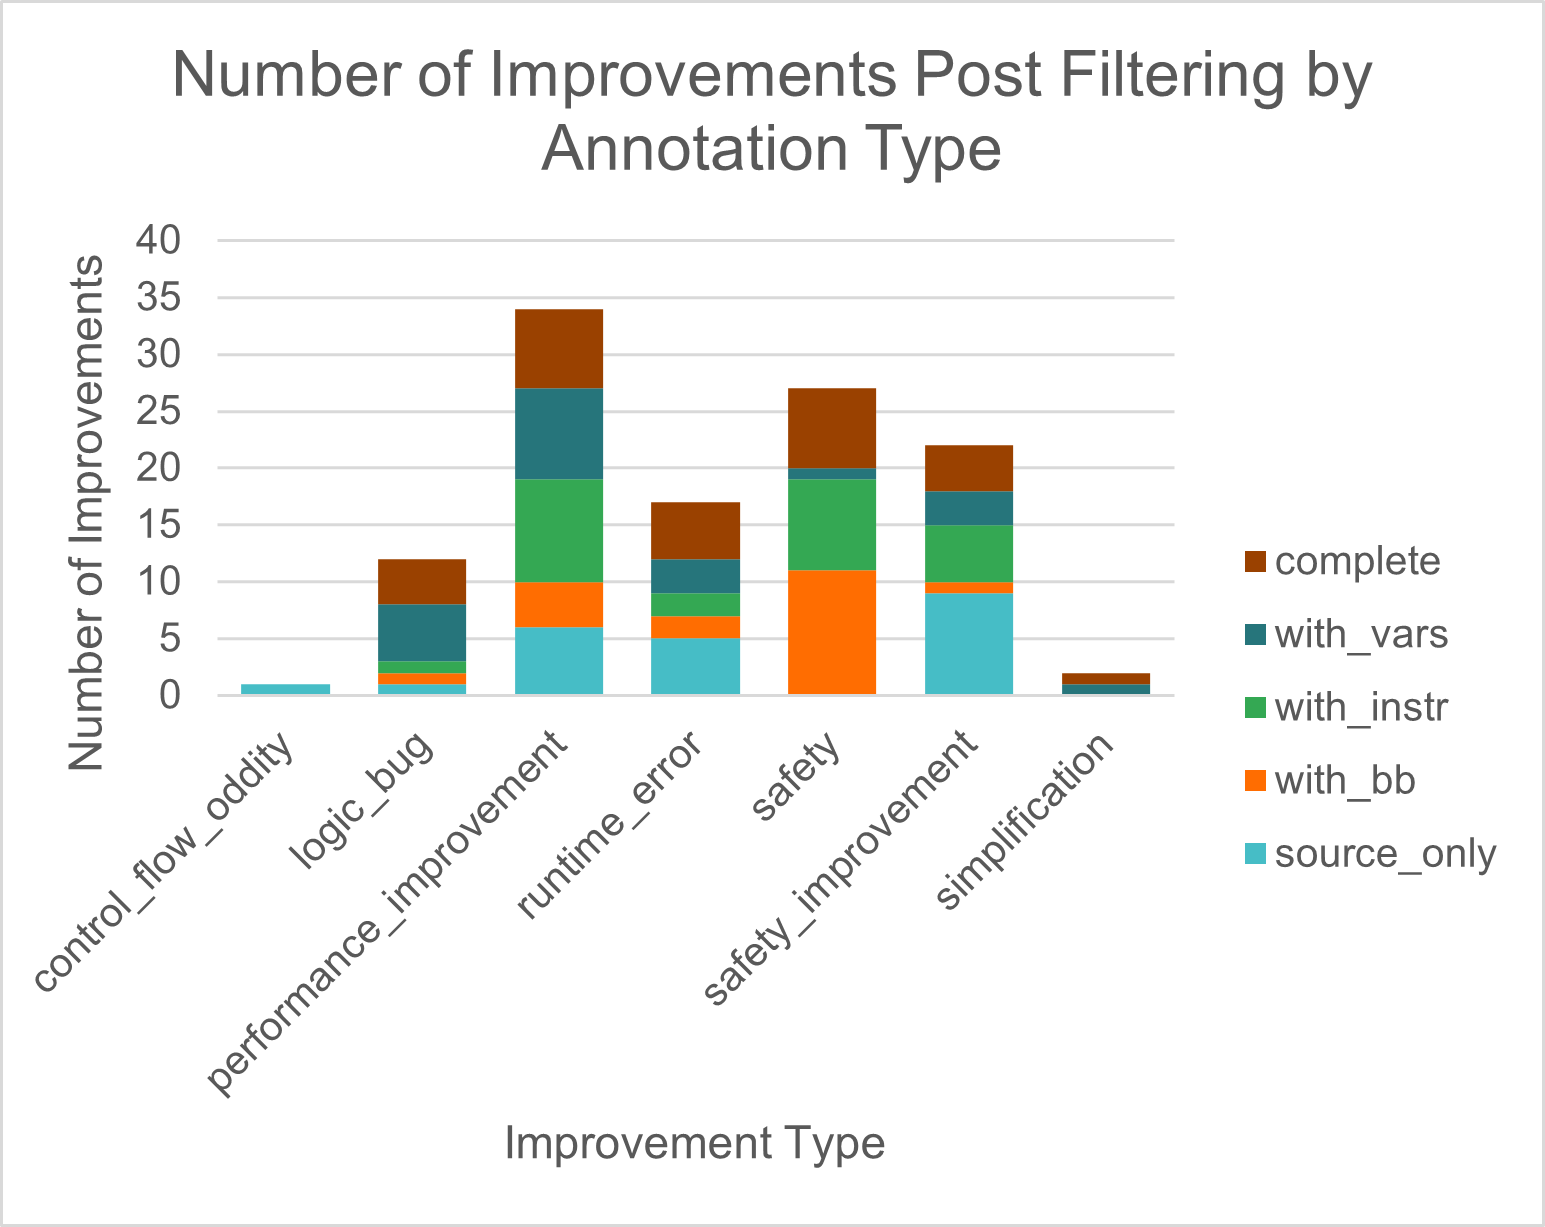
\includegraphics[width=0.8\linewidth]{images/PostFiltering.png}
    \caption{Number of improvement recommendations across each annotation type.}
    \label{fig:filtered}
\end{figure}

The responses from the LLM for each benchmark on each type of code annotation were recorded.
These responses were then filtered.
Responses that did not actually provide useful information or where the improvement\_desc did not correlate with the type\_of\_improvement were filtered out.
Figure~\ref{fig:filtered} shows the results after this filtering occurred.
There were 7 improvement types provided by the model, although some were highly related such as `safety' and `safety\_improvement'.
It is worth noting that, for all common improvement types, the annotated source code prompts received more improvement recommendations than the unannotated prompt.
This is clearer especially if the `safety' and `safety\_improvement' categories are considered together.
Of the annotated prompts, the weakest performing was the with\_vars annotation.
It does not appear particularly useful to the LLM to receive just information on common variable values at points in the code.
The annotated prompt type that yielded the most feedback was the complete annotation.
With all forms of information, the LLM was not overwhelmed, as was initially feared, but performed optimally.

\begin{figure}
    \centering
    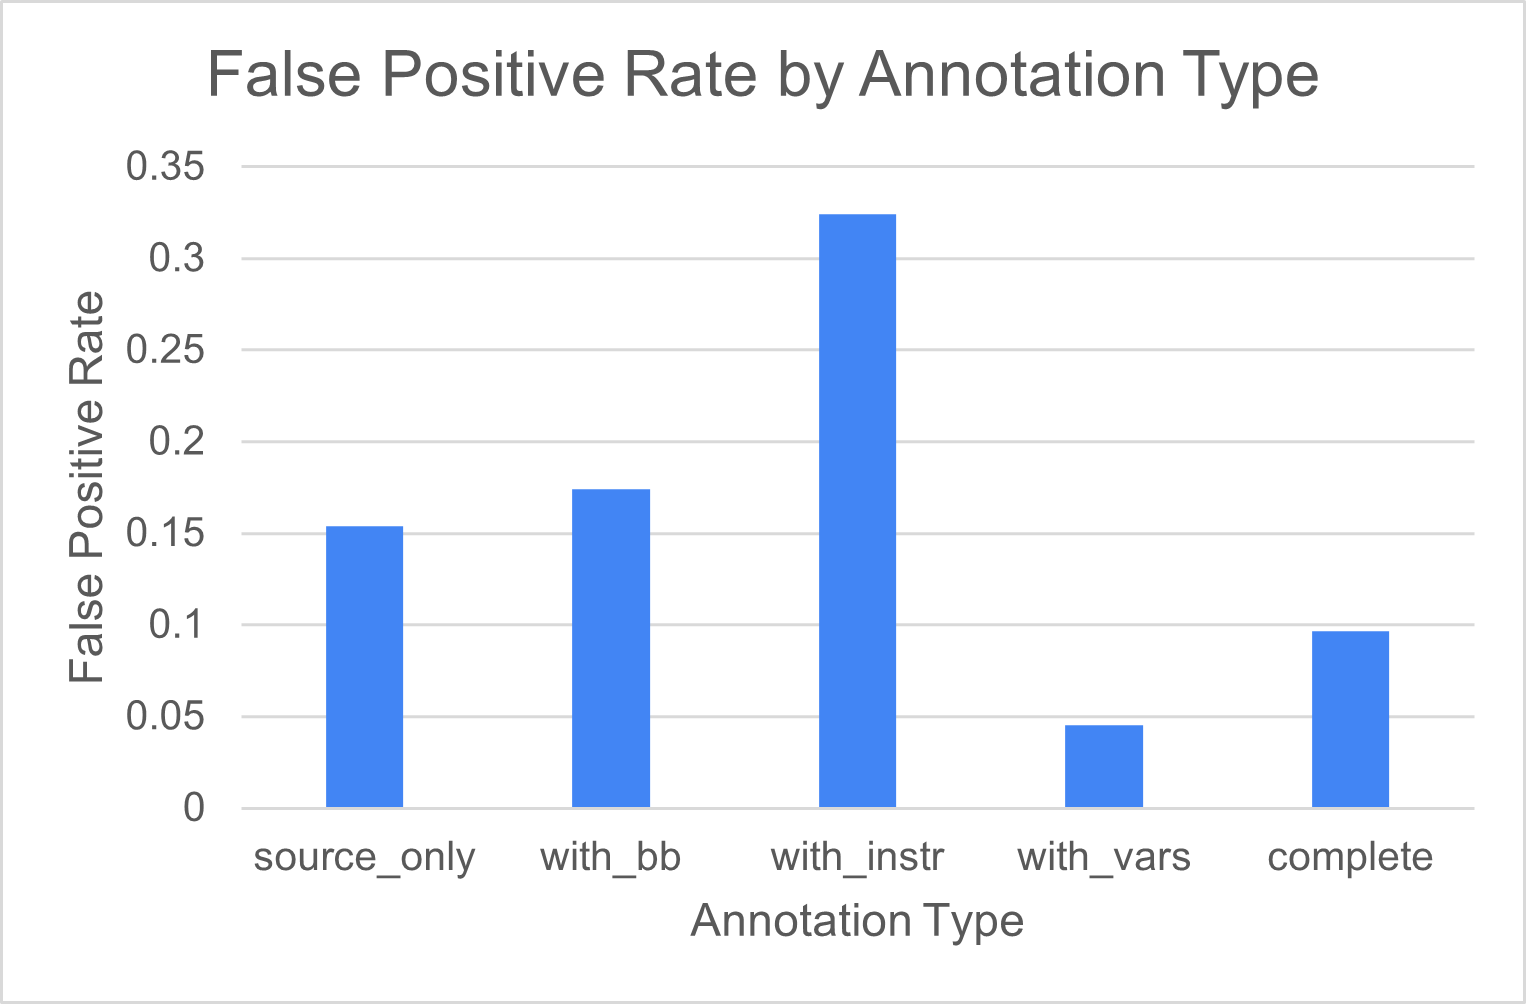
\includegraphics[width=0.8\linewidth]{images/FalsePositiveRate.png}
    \caption{Rate of inaccurate or unhelpful recommendations by the LLM categorized by annotation type.}
    \label{fig:falsePositive}
\end{figure}

The false positive rate, or how often the individual improvement recommendations were not accurate or not useful, was analyzed for each annotation type, and these results can be seen in Figure~\ref{fig:falsePositive}.
All annotation types had significant false positive rates of at least 4\% and often over 10\%.
The bytecode instruction code annotation had a very significant false positive rate.
This was partially due to it sometimes providing feedback that there was "no issue" in a particular portion of code, which is not relevant if the prompt is seeking improvements.
Thus, the false positive rate can be understood as the rate of not only incorrect information but also useless information.
This is information that the user of GinS would have to know to filter out, and this false positive rate is very significant for someone who would consider using this system.

\subsection{Smart Assertions Performance}
Smart asserts were also tested on the 7 benchmarks that were used to test GINS, with benchmark containing test cases that would discover a bug, resulting in a smart assert to fail.
The quality of the LLM's analysis was manually tested in three different categories:

\begin{itemize}
    \item \textbf{Diagnosis Accuracy} If the LLM could correctly identify the specific root cause of the failure.
    \item \textbf{Fix Correctness} If the fix provided by the LLM was correct.
    \item \textbf{Explanation Clarity} If the textual explanations provided by the LLM were clear, concise, and easy to follow, even if the analysis itself was incorrect.
\end{itemize}

Each benchmark was rated on a scale between 0 and 2:

\begin{itemize}
    \item[0:] Incorrect / Unclear 
    \item[1:] Partially Correct / Acceptable
    \item[2:] Correct / Clear
\end{itemize}

\begin{figure}
    \centering
    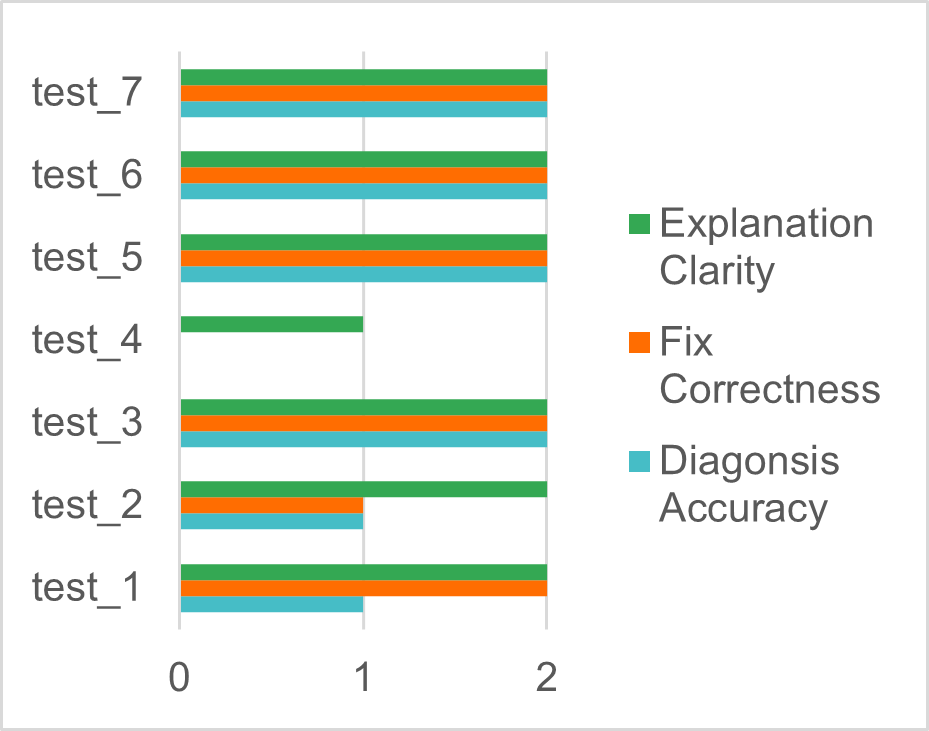
\includegraphics[width=0.8\linewidth]{images/smartAssert.png}
    \caption{Smart assert response analysis on 7 benchmark tests}
    \label{fig:smartAssert}
\end{figure}

Smart asserts were able to correctly identify the root cause of errors in 5 out of the 7 benchmarks, and partially identify the error type in another. The primary exception was a heavy misdiagnosis in benchmark 4, where the analysis suggested that the test cases used were incorrect, instead of pinpointing the bug that existed in the code's logic.
When these root causes were correctly or partially identified by smart assert, the corresponding fix provided in the response was also found to be correct and addressed the underlying issue.
In terms of clarity, despite the inaccurate conclusion in one benchmark, the explanations provided by the LLM were consistently rated as very clear and easy to follow.
We also observed for benchmarks 5, 6 and 7, the analysis benefitied from the runtime variable tracking information included in the prompt. It explained step by step what variable values existed in iterations of the code, noting what bugs caused discrepencies between the program output and the expected output.

\subsection{GinS Overhead}
The overhead of GinS was also analyzed.
\begin{figure}
    \centering
    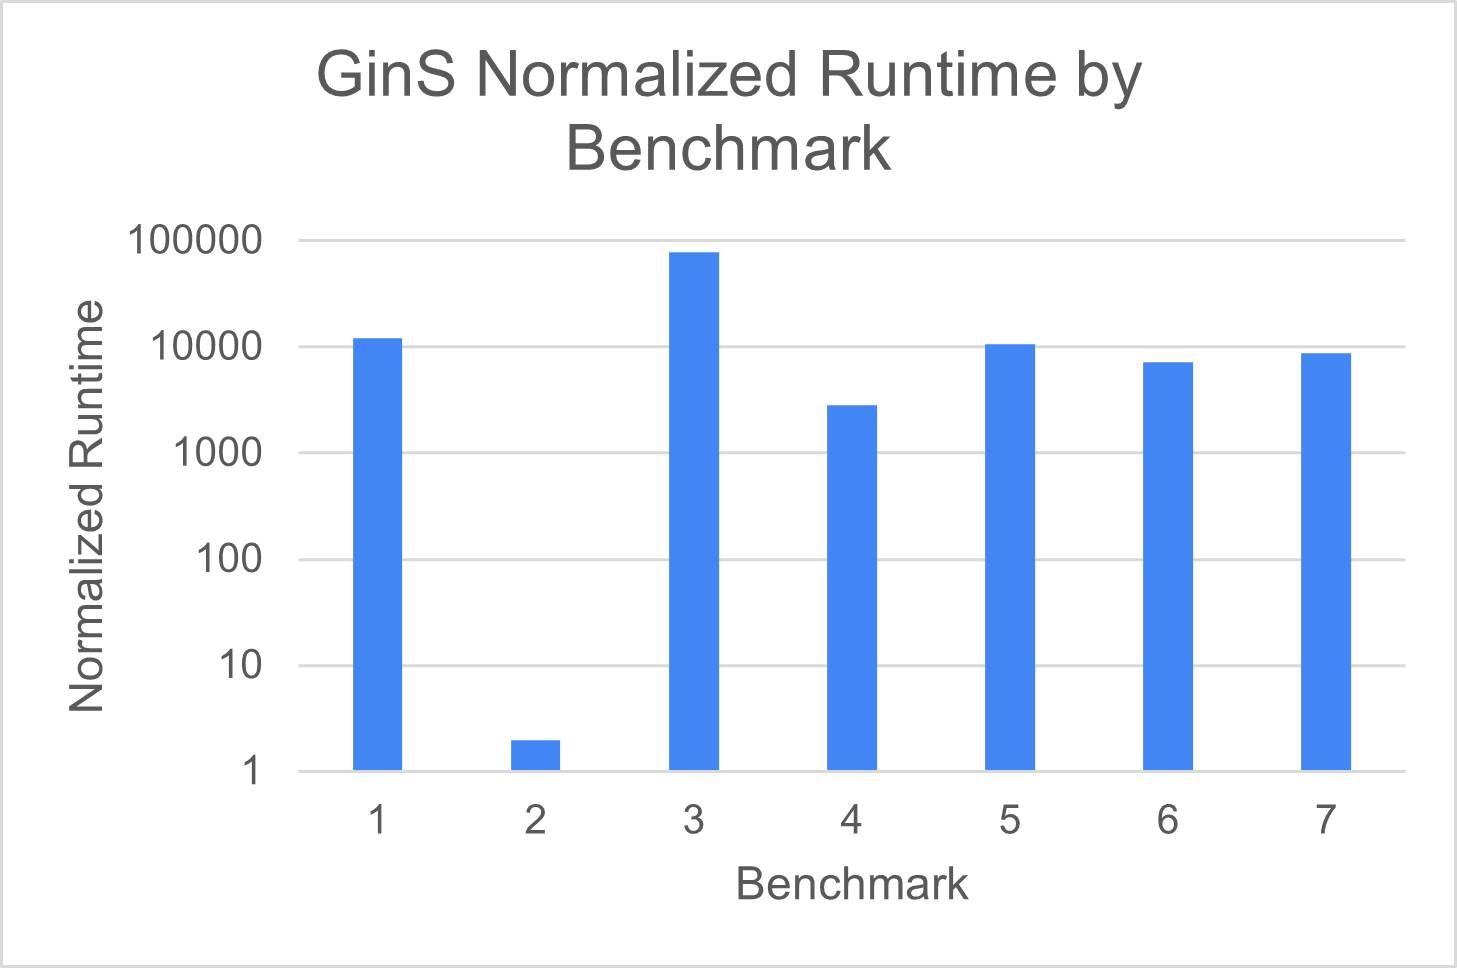
\includegraphics[width=0.8\linewidth]{images/Time.png}
    \caption{GinS runtime normalized to runtime without GinS across benchmarks.}
    \label{fig:time}
\end{figure}

One major consideration in the usefulness of GinS is how significantly GinS affects runtime.
The GinS runtime for each benchmark is compared to the runtime without GinS in Figure~\ref{fig:time}.
It is clear from this figure that GinS increases runtime by a number of orders of magnitude for most benchmarks.
It is worth noting that because testing was limited to relatively short running programs, the accuracy of these overhead numbers is unknown for longer running programs.
These programs ran on the scale of hundreds of nanoseconds, and the prompting of the LLM was usually on the scale of half a second or seconds.
Thus, this overhead explosion is likely greatly reduced for programs that run for times on the scale of an LLM prompting.
However, it is clear that GinS is not an efficient tool for short running programs such as those used as benchmarks.
The use of longer running programs is discussed in the conclusion.

\begin{figure}
    \centering
    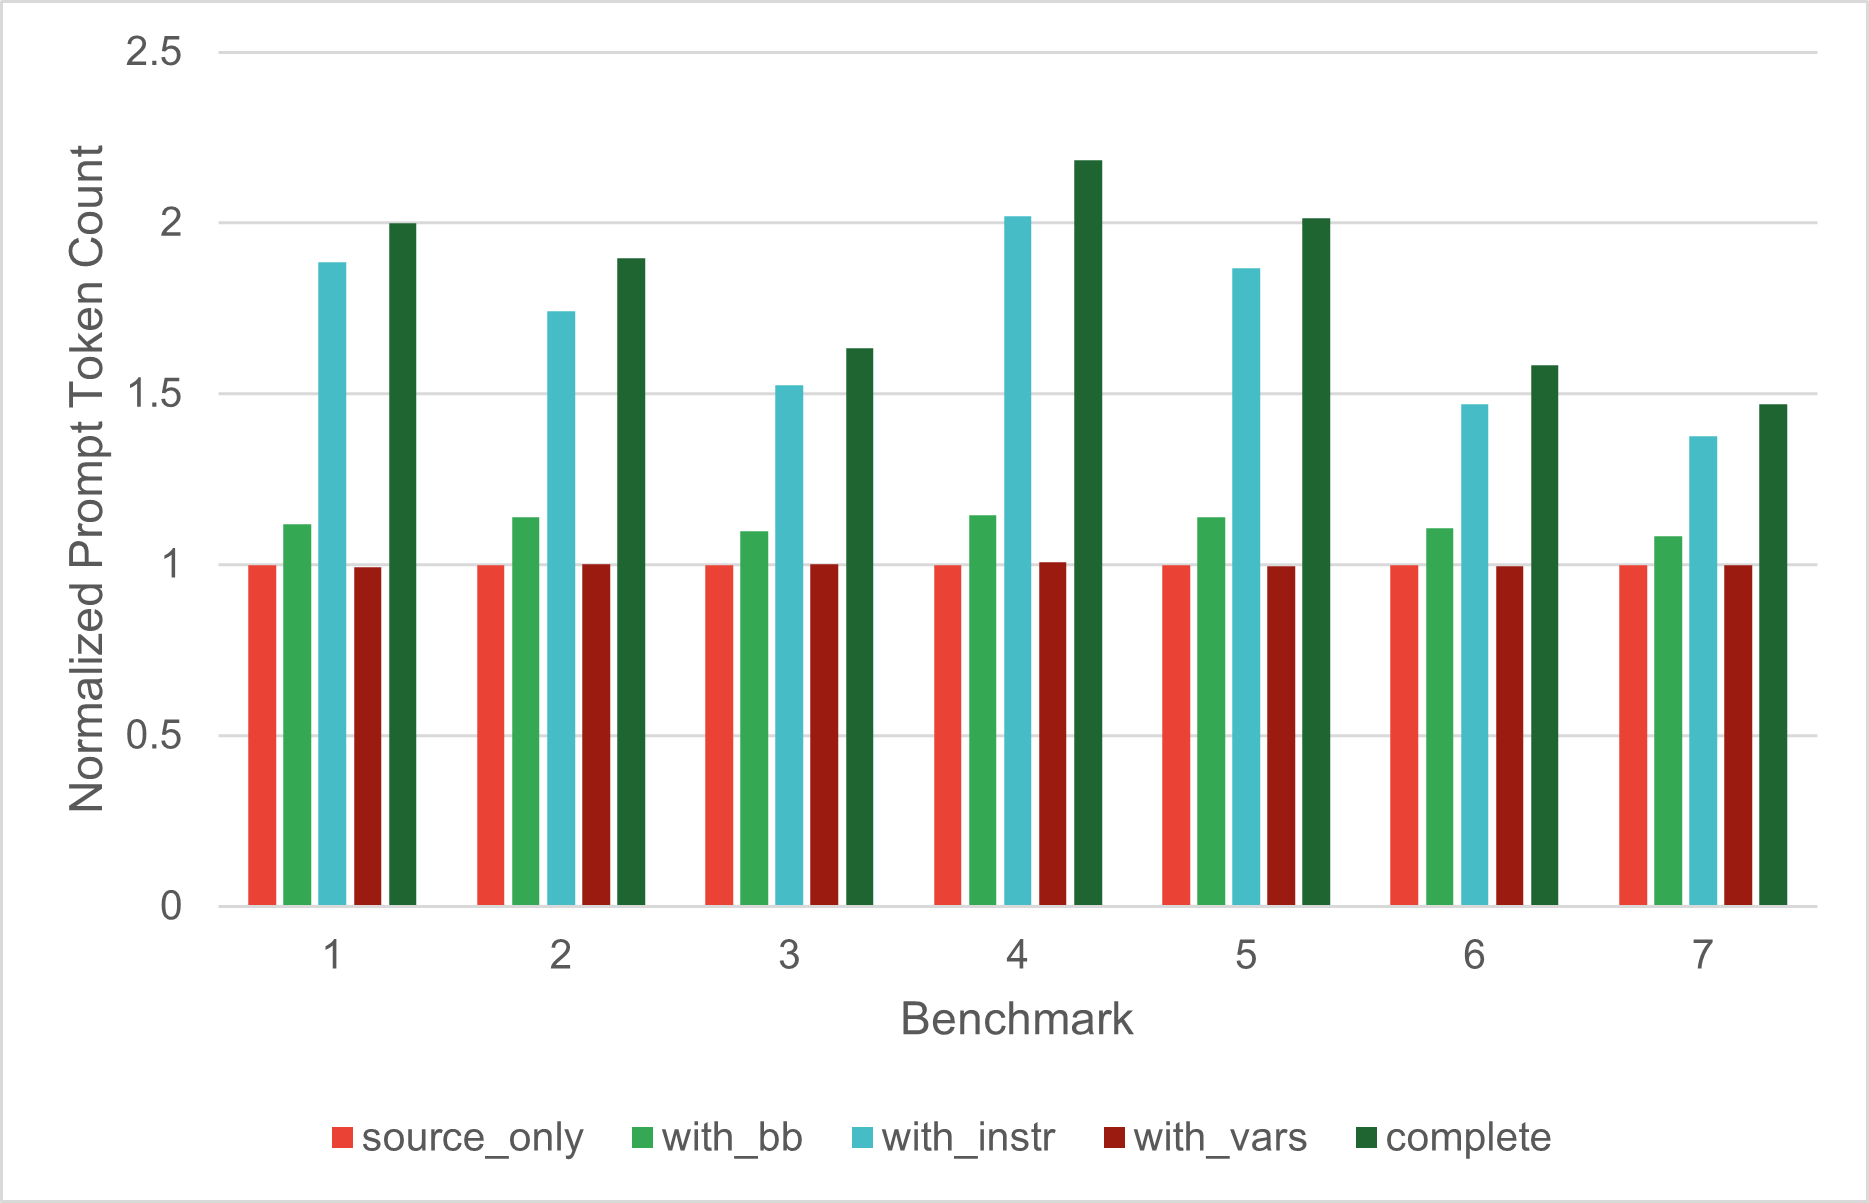
\includegraphics[width=1\linewidth]{images/PromptCost.png}
    \caption{Prompt token count for each annotation type normalized to source code prompt length across benchmarks.}
    \label{fig:prompt}
\end{figure}

Another form of overhead for GinS is the size of prompts sent to the LLM, and the size of the LLM's responses.
Figure~\ref{fig:prompt} shows the prompt size as token count across each benchmark.
These token counts are normalized to the prompt that contained no code annotations as this was a baseline for the prompt size.
The basic block and variable value annotations had rather negligible effects on prompt size, while the instruction annotations had a major impact.
These often reached at least a 50\% increase in prompt length.
Since the complete annotation is the combination of all other annotations, it achieved the highest prompt length, but it was usually at a similar scale to the instruction annotations.
Prompt length is a concern due to LLM's having a limited context window.
For longer running applications, the source code itself may be longer than the context window, and so the annotated code would be even more likely to exceed this limit.
However, as models are continually refined and released, the context window will also likely increase.
This in turn may reduce the relevancy of this overhead metric.

\begin{figure}
    \centering
    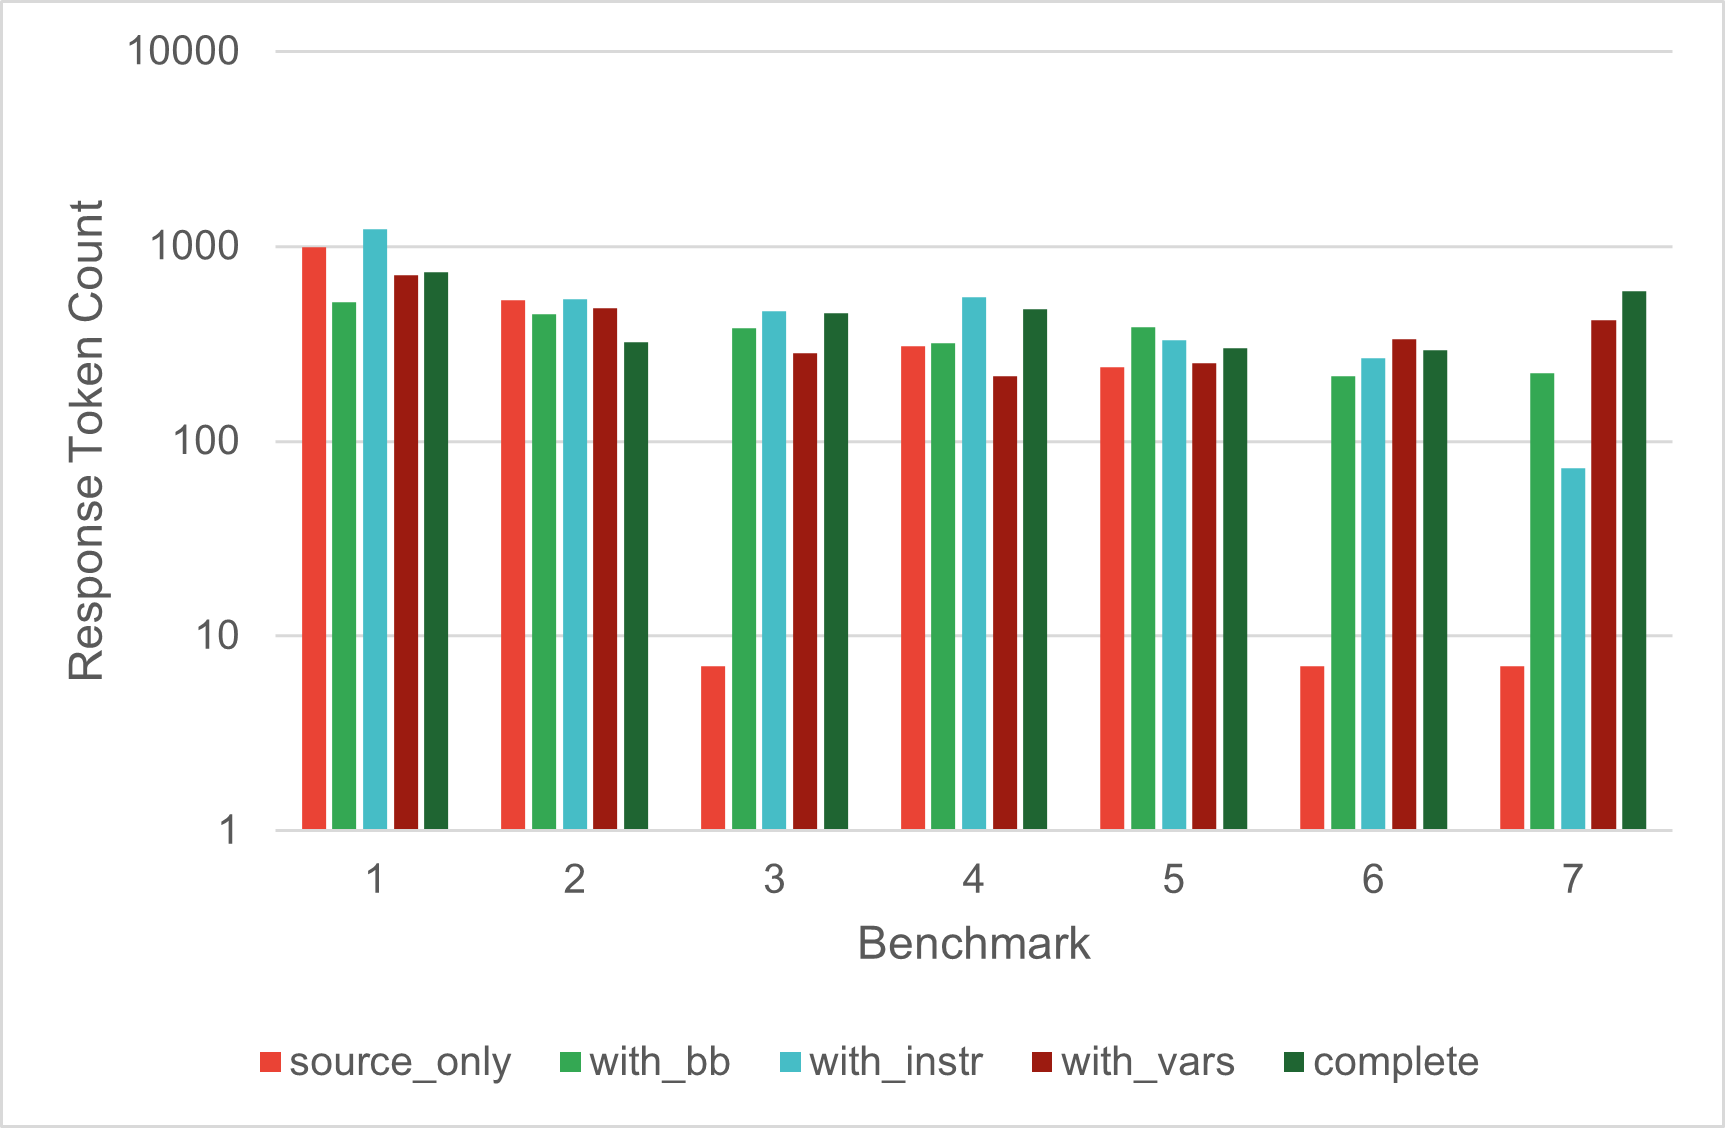
\includegraphics[width=1\linewidth]{images/ResponseCost.png}
    \caption{Response token count across benchmarks for each annotation type.}
    \label{fig:response}
\end{figure}

The final overhead metric that was tested was the size of the response.
The comparison in response length can be seen in Figure~\ref{fig:response}, although these token counts are not normalized since there is no default response length.
Response lengths are fairly similar for each annotation type across benchmarks with a few exceptions.
The unannotated prompt received very short replies for a few benchmarks, namely 3, 6, and 7.
This short response represents an empty response for these benchmarks.
The LLM did not provide relevant feedback for these benchmarks as it did not appear to have information worth sharing for these benchmarks.
Each response seemed to be in the hundreds of tokens, and very rarely approached or exceeded 1000 tokens.
It is worth noting that this form of overhead is directly correlated with the usefulness of GinS.
A larger LLM response that is not full of irrelevant or incorrect information is not necessarily a worse response.
Reducing response size too significantly can result in greatly reducing the amount of information able to be conveyed by the LLM.
Thus, while this is technically a form of overhead, it is not necessarily a design goal to reduce this overhead significantly, and it may be a goal to increase it as long as that corresponds to more productive feedback from the LLM.


\section{Conclusion and Future Work}
The current GinS system leads to more useful feedback from an LLM on how to improve one's code.
This was accomplished by developing three types of code annotations and then considering them individually and then combining them.
These three annotations were basic block and cfg annotation, bytecode instruction annotation, and common variable values annotation.
Structured output supported by Gemini-1.5-pro was used to receive code improvement recommendations in a useful format.
The feedback from the LLM was mostly useful, but it did provide excess or unhelpful information at a rate of about 10\%.
Notably, GinS, in its current form, has rather high token cost in comparison to current contex windows, and also has an extremely large time overhead.
These issues result in GinS needing notable effort to make it more useful.

Testing GinS on larger programs that run for longer times would yield valuable results.
This could show that the time overhead is much less significant for programs that run on the time scales of or greater than that of an LLM request.
This also could show that current context windows are not great enough to handle the annotated source code or even the regular source code of a larger program.
We were unable to test GinS on larger programs due to the fact that GinS, in its current form, is unable to track and understand unhashable types such as lists.
Since many unhashable types are requisite for any long Python program, this issue highly limited the benchmarks that we were able to use.
Thus, the first step in future work for GinS would be to fix this tracking issue for GinS, and then to use that unlocked potential to test it on longer running programs.

%%
%% The next two lines define the bibliography style to be used, and
%% the bibliography file.
\bibliographystyle{ACM-Reference-Format}
\bibliography{references.bib}

%%
\end{document}
\endinput
%%
%% End of file `main.tex'.
